% !TeX root = ../../thesis.tex
\chapter{Introduction}\label{ch:introduction}

\newglossaryentry{eids}{name={EIDs},description={Emerging infectious diseases}}

Infectious diseases are now emerging or reemerging almost every year.
This trend will continue because a number of factors, including increased global population, aging, travel, urbanization, and climate change, favor the emergence, evolution, and spread of new pathogens \cite{bloom2017emerging}.
Many of these pathogens represent a clear and eminent threat to public health, as the ongoing corona virus disease (COVID-19) pandemic caused by severe acute respiratory syndrome corona virus 2 (SARS-CoV-2) has made brutally clear, as well as a tremendous burden on global economies.
Other examples from the last few years include the emergence of West Nile \cite{hadfield2019twenty}, H5N1 \cite{imai2018diversity}, H1N1 \cite{bedford2015global}, Ebola \cite{dudas2017virus}, Zika \cite{fauci2016zika, faria2016zika} and Lassa \cite{kafetzopoulou2019metagenomic}.
Demographic forces amplify the risks associated with such emerging infectious diseases (\gls{eids}).
The global population is expected to grow to 8 billion in the near future, with nearly 60\% of the population living in relatively crowded urban areas.
Among \gls{eids}, viral pathogens, particularly RNA viruses, stand as major concerns, owing to their high rates of nucleotide substitution and capacity to adapt to new hosts.
Viral sequence data are invaluable for characterising these pathogens.
Analysing the historical information contained in viral genomes contributes to better insight into viral emergence and early transmission dynamics, even before systematic epidemiological surveillance initiates.

\section{Phylogenetics}

Molecular phylogenetic inference is a particularly powerful tool available to scientists interested in inferring pathogen dynamics.
This is a methodology by which the shared evolutionary history of a set of genomic sequences, sometimes referred to as taxa, is hypothesized based on genomic similarity.
Phylogenetic methodologies come in many different forms, ranging from simple heuristics that approximate phylogenetic relationships based on the number of observed differences between sequences \cite{felsenstein2003inferring} to highly complex models that use demographic and geographic population structure as well as state-of-the-art models of evolution to inform phylogenetic inference \cite{dudas2018mers}.
Additionally, phylogenetic analyses may be combined with other methodologies (e.g. methods in population genetics \cite{felsenstein2003inferring} or epidemiology \cite{black2020ten}) to provide insight into the relationship between evolutionary dynamics and other processes.

\newglossaryentry{mrca}{name={MRCA},description={Most recent common ancestor}}

Phylogenetic methods can help reveal many features of a set of related taxa.
The most frequent use of these methods is to construct a phylogenetic tree: a bifurcating (or sometimes multifurcating) representation of the inferred evolutionary history of a set of contemporary taxa---represented as tips or leaves of the tree---with inferred shared ancestors represented by internal nodes where two or more branches of the tree meet, eventually coalescing at the most recent common ancestor (\gls{mrca}) of all the taxa in a dataset.
Such trees often use length of branches to represent genetic distance between nodes.
A more useful representation of evolutionary history can be found by rescaling branch lengths along a tree according to a mutation rate which provides a mapping between genetic distance and time, allowing the phylogeny to be represented as a function of time.
Phylogenetic trees can also be used to infer the shared mutation history of a set of sequences, thereby allowing the reconstruction of inferred ancestral genomes.
Similar methods may be used to reconstruct the ancestral states of various discrete or continuous traits associated with the taxa of the tree.
Common examples of these types of analyses include analyses of particular phenotypes of interest and phytogeographic analyses that treat sequence sampling locations as traits and aim to reconstruct the spatiotemporal spread of pathogens.
Finally, phylogenetic methods often hypothesize a link between population dynamics and tree shape---formalized through coalescent theory \cite{Kingman1982}---whereby small populations are expected to have relatively high rates of branching (and therefore relatively short branch lengths) compared to larger populations.
Visual examples of all of these aspects of phylodynamic analyses are illustrated in Fig.~\ref{fig:phylogeneticsOverview} \cite{pybus2009evolutionary}.

\begin{figure}[ht]
  \centering
  \medskip
  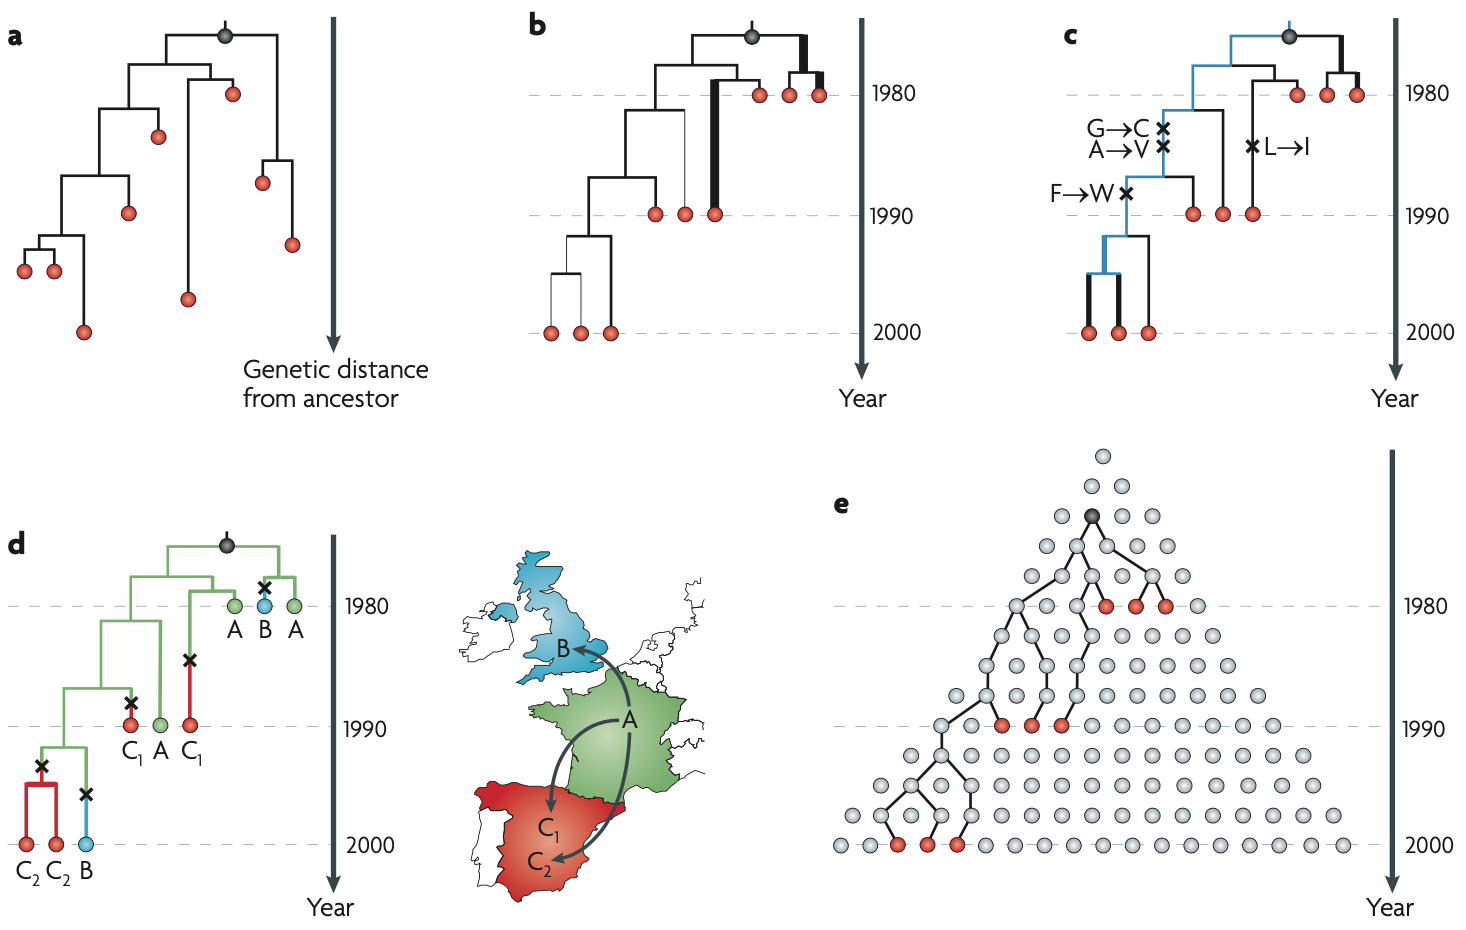
\includegraphics[width=.9\textwidth]{rambautFig}
  \caption[Applications of phylogenetic analysis]{Key concepts in phylodynamic analysis.
  a) Molecular phylogenies from viral gene sequences are typically rooted and bifurcating.
  b) A molecular clock allows to define a relationship between genetic distance and time, with unusually fast or slow evolving lineages are shown as thick or thin lines, respectively.
  c) Phylodynamic data can also highlight the evolution through time of mutations that may reflect viral adaptations; of particular interest are the replacement mutations that are found on the persisting phylogenetic ‘backbone’ that represents the ancestor of future virus populations (blue branches), as opposed to those occurring on branches that die out (black branches).
  d) Temporal phylogeographic inference is used to reconstruct the history of pathogen spread, so that each branch is labelled with its estimated geographic position.
  e) Coalescent analyses incorporate an explicit model of the sampled pathogen population.
  The increasing width of each row therefore reflects the growth of the epidemic through time. Starting from the sampled infections (red), the sampled lineages (black lines) can be traced back through unsampled infections (grey) to the common ancestor (black circle).
  (\textit{Figure credit: Pybus \& Rambaut 2009} \cite{pybus2009evolutionary})
  }
  \label{fig:phylogeneticsOverview}
\end{figure}

\newglossaryentry{hbv}{name={HBV},description={Hepatitis B virus}}
\newglossaryentry{lasv}{name={LASV},description={Lassa virus}}

One particularly useful application of phylogenetics is in the analysis of viral pathogen outbreaks.
Viruses represent unique study systems for both the theoretical development of phylogenetic methodologies and the implementation of phylogenetic analyses in settings with tangible public health impact.
In addition to their ubiquity and high profile within the human population, viruses prove highly suitable for phylogenetic inference because of their fast evolutionary rates, relatively small genomes, and frequent adherence to the assumptions of a single evolutionary history.
Phylogenetic methods have often been used to perform \textit{post hoc} analyses of viral outbreaks, however significant work is still required before such methods can be used to inform public health responses in ``real-time'' during an ongoing epidemic.
In this thesis, we describe phylogenetic analyses of two viral pathogens---hepatitis B virus (\gls{hbv}) and Lassa virus (\gls{lasv}).
We use these analyses to illustrate the use of current phylogenetic and phylogeographic analysis in performing retrospective analysis, and to provide a framework for novel ``online'' phylogenetic analyses that can be performed in real-time during a viral epidemic.

\section{Measurably evolving populations and temporal signal}

While performing phylogenetic analyses, we are often interested in how populations evolve as a function of time, rather than as a function of genetic distance.
To this end, we seek a way to correlate differences in our input data (i.e. genetic distance) with time.
We do this by assuming that mutations accumulate along the branches of a phylogenetic tree according to some rate, which can be posited to hold a constant value across the entire phylogeny \cite{brown2011rate}, or can vary by branch according to different statistical models \cite{drummond2006relaxed, drummond2010randomLocal}.
We refer to this rate as a ``clock rate''---generally represented in units of substitutions per site per year.
The clock rate can be used to rescale the branches of a phylogeny from units of genetic distance to units of time.

\newglossaryentry{mep}{name={MEP},description={Measurably evolving population}}
Historically, such clock rate calculations were produced using informed estimates of divergence times between two known lineages using fossil calibration\cite{smith2010birds, near2005turtles}---a process whereby internal node times were set to an externally-supplied date of divergence.
While this approach works well for reconstructing phylogenies for eukaryotic species whose extant genomes are more-or-less isochronous and fossil records exist to date ancient divergences, it has limited use in the inference of molecular clocks in viruses, where known divergence times may be much more limited.
Indeed, it is frequently impossible to provide accurate prior estimates of historical divergence times, and we instead wish to infer molecular clock rates directly from heterochronous (i.e. sampled over long periods of time) sequences.
We call the existence of sufficient statistical power from heterochronous sequence data to determine a molecular clock rate ``temporal signal'', and we refer to a population from which we can observe a statistically significant number of mutations through time a ``measurably evolving population'' (\gls{mep}) \cite{drummond2003measurably}. %GB: how can this be deemed to be 'statistically significant'?
In general, there are two sources from which we can observe \gls{mep}s: populations with available ancient genomes, and rapidly evolving RNA viruses.
Analysis of ancient genomes has proven to be an effective way of inferring the phylodynamics of eukaryotic populations \cite{shapiro2004bison}. %GB: if there is still room, I would be tempted to provide more information regarding this example, and perhaps the key figure from that paper

\section{Bayesian phylodynamic inference}

In this thesis, we specifically use Bayesian methodologies of phylogenetic inference.
Unlike many other approaches, including maximum-likelihood inference, Bayesian methods do not assume that the parameters which govern statistical models take a single-point value, but rather come from a posterior probability distribution.
Such methodologies are also informed by hypotheses of these parameter distributions provided \textit{a priori} by researchers---referred to as parameter prior distributions.
Bayesian methodologies are particularly well suited to phylogenetic methods in several key ways.
Firstly, they allow researchers to create strongly supported estimates of evolutionary histories that account for uncertainty in the phylogenies and in other model parameters.
Additionally, Bayesian phylogenetic methods afford researchers the opportunity to infer many different parameters of interest (e.g. mutation rates, effective population sizes, and migration rates) jointly with the phylogeny.
Finally, for many different evolutionary models algorithms for performing Bayesian phylogenetic inference are well defined and implemented efficiently, allowing tractable computation.

\newglossaryentry{mcmc}{name={MCMC},description={Markov chain Monte Carlo}}
To perform Bayesian analyses it is frequently necessary to compute very large, high-dimensional integrals to produce exact posterior distributions; this task is unfortunately typically analytically intractable.
However, this hurdle can be overcome by simulating a Markov chain whose stationary distribution is the desired posterior distribution.
This approach is known as Markov chain Monte Carlo (\gls{mcmc}) and can be exploited to numerically approximate posterior distributions of phylogenetic models.

% MG: this entire paragraph needs to be rewritten. It is poorly and sometimes inaccurately explained.
The implementation of such methods works according to a modified Metropolis-Hastings algorithm.
First, a starting value for each parameter of interest is randomly drawn from its prior distribution or set to a pre-specified value.
%For numeric parameters this takes the form of one or more numbers being generated randomly, and a random tree topology is used as the initial tree.
A likelihood for the model can then be calculated, conditional on the current values of the model parameters.
A new ``proposal'' set is then generated by stochastically permuting the original parameter set according to a various parameter-specific transition kernels.
If the proposal set yields a higher likelihood than the initial set, it is accepted as the new candidate set.
If they have a likelihood lower than the initial candidate set, they will be accepted with probability proportional to the ratio of their likelihoods.
This process is then repeated, until a stable parameter and tree set are found.
This stable set is considered to be the posterior distribution from which we would like to sample.
We continue to repeat the process, recording the state of the chain at regular intervals, until the posterior has been sufficiently explored.
At that stage, which can take days or even weeks to reach (but see section~\ref{sec:ess}), we can stop our Bayesian analysis and construct summaries of all parameters of interest.

\subsection{Statistical and computational challenges}

One of the major challenges of phylogenetic inference that can lead to very time-consuming analyses is the vast size of the state space of potentially inferred variables.
The size of ``tree space''---the set of all possible phylogenetic trees for a given dataset---scales at the rate $\frac{(2n-3)!}{2^{n-1}(n-1)!}$.
This is far too large to exhaustively explore for the datasets that researchers are interested in; for a dataset consisting of only thirty taxa, the number of possible rooted, labeled phylogenies numbers over $10^{38}$ \cite{felsenstein2003inferring}.
For the datasets that we explore in this thesis---ranging in size to 769 taxa---this number grows to vastly overshadow the number of atoms in the observable universe.
As such, exhaustively exploring this space is impossible, and traversing this space algorithmically can still take considerable time.

\subsection{Effective sample size and burn-in}
\label{sec:ess}
\newglossaryentry{ess}{name={ESS},description={Effective sample size}}

Bayesian phylogenetic inference of large, complex datasets can hence take upwards of a month of constant computational time before a chain achieves convergence and has adequately explored the full posterior distribution.
During this time, we sample the constructed Markov chain at fixed intervals by recording the state of all parameters of the chain.
We quantify how thoroughly the posterior has been sampled using a metric known as the effective sample size (\gls{ess})---a measure of the number of effectively independent draws from the posterior distribution that the Markov chain sample is equivalent to.
Because sequential samples of the chain's state are frequently highly correlated, we find \gls{ess} to be an appropriate metric for how fully the \gls{mcmc} has explored the posterior distribution of interest.
While there is no theoretical foundation for using a specific cut-off value when computing the \gls{ess}, we generally seek to accumulate \gls{ess} values over 200 for each parameter of interest as a decent trade-off between length of computation and the number of independent samples collected for a specific parameter.

A significant amount of computational time is consumed by the chain moving from where it began in state space toward the posterior distribution---a period referred to as ``burn-in''.
Because the chain is rapidly traversing parameter space during this period all samples are correlated, and we are therefore unable to accumulate any \gls{ess} during this time.
Indeed, the entire burn-in period is discarded prior to analysis.
The burn-in period can take upwards of 10\% of the total computation time.
A major computational issue stemming from the burn-in period is that the time spent in burn-in can only be mitigated by specifying prior distributions that are strongly informative of the posterior distribution.
This means that even if identically parameterized chains are run in parallel the burn-in period must take place for each independent run, significantly lowering the utility of chain-level parallelization.

\subsection{BEAST}

\newglossaryentry{beast}{name={BEAST},description={Bayesian Evolutionary Analysis Sampling Trees}}
For the analyses described in this thesis, we make use of the software package Bayesian Evolutionary Analysis Sampling Trees (\gls{beast}) 1.10 \cite{suchard2018bayesian}.
\gls{beast} is an easy-to-use software package in which many Bayesian phylogenetic models---and their associated priors and transition kernels---have been implemented and optimized such that analyses on large datasets may be easily specified and run efficiently on a wide variety of computing resources.
%This tool mostly implements Bayesian phylogenetic inference via \gls{mcmc} but recent developments have started exploring the use of Hamiltonian Monte Carlo approaches. %MG: HMC is an MCMC method
Analyses in \gls{beast} are facilitated by hardware optimization libraries \cite{ayres2019beagle}, as well as a large suite of utility programs that make running analyses in parallel and quickly interpreting results feasible.

\section{Viral pathogens}
Viral pathogen outbreaks are a particularly useful study system for Bayesian phylogeneticists because their relatively small genomes typically allow for tractable computation.
The rapidity with which viruses move though populations and their fast evolutionary rates give many viral pathogens rather strong temporal signal, and therefore make them good candidates for Bayesian phylogenetic inference.
Viral pathogens make interesting study systems because of the large influence that they exert on human quality of life.
Viruses frequently cause human suffering and death, both as endemic diseases (seasonal influenza, hepatitis, etc.) and the agents behind sudden disease epidemics (Zika, Ebola, Lassa).
Indeed, viruses have been responsible for the majority of the most deadly pandemics of the last century (1918 Spanish influenza, 2009 Swine flu, COVID-19).
Even when they do not cause large-scale epidemics or global pandemics, or when they do not cause death, viruses can still cause vast amounts of human suffering though localized, small-scale outbreaks that cause severe health problems for those that they infect.
In this thesis, I present the results of Bayesian phylogenetic analyses of two separate viral pathogens: hepatitis B virus (\gls{hbv}) and Lassa virus (\gls{lasv}).


\subsection{Hepatitis B virus (HBV)}

\gls{hbv} has infected over two billion people worldwide, and puts over 350 million people at risk of cirrhosis and liver cancer \cite{kane1995global}.
The virus is classified into eight different genotypes based on genomic sequence divergence.
These genotypes show strong ethnospatial patterns, and are often correlated directly to the region of the world where they are most prominent \cite{schaefer2007hepatitis}.
\gls{hbv} consists of two partially overlapping strands of DNA (Fig.~\ref{fig:hbvGenome}).
The long strand ranges from 3,020--3,320 bases in length, while the short strand ranges from 1,700--2,800 nucleotides long, depending on genotype \cite{kay2007hepatitis}.

\begin{figure}[ht]
  \centering
  \medskip
  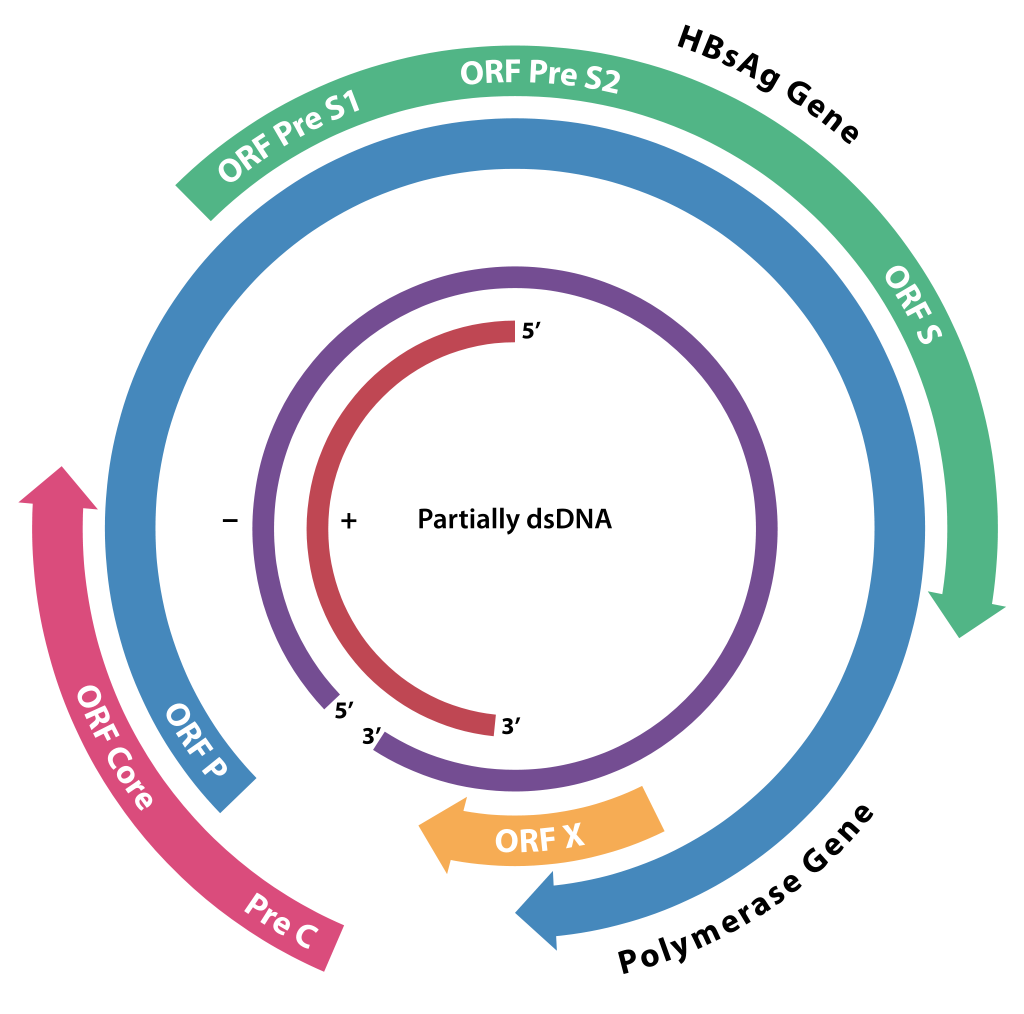
\includegraphics[width=.6\textwidth]{hbv_genome_schematic}
  \caption[Scematic of the HBV genome]{The \gls{hbv} genome consists of two partially overlapping strands of DNA. The long strand (purple) is roughly 3 kb in length and circular, while the shrot strand (red) is roughly 2.2 kb in length. Between the two strands there are four identified open reading frames. (\textit{Figure credit: Wikimedia Commons} \cite{HBVwiki})}
  \label{fig:hbvGenome}
\end{figure}

\subsection{Lassa virus (LASV)}

Lassa virus (\gls{lasv}) is the causative agent of Lassa fever, a viral hemorrhagic fever that infects 300,000--500,000 people anually and causes 54,000--90,000 deaths yearly \cite{lianaThesis, asogun2012molecular}.
\gls{lasv} has a genome that is divided into two segments: a large (L) segment approximately 7.5 kb in length, and a small (S) segment approximately 3.5 kb in length.
The L segment encodes genes \textit{Pol} and \textit{Z}, while the S segment encodes genes \textit{GPC} and \textit{NP} (Fig.~\ref{fig:lasvGenome}).

\begin{figure}[ht]
  \centering
  \medskip
  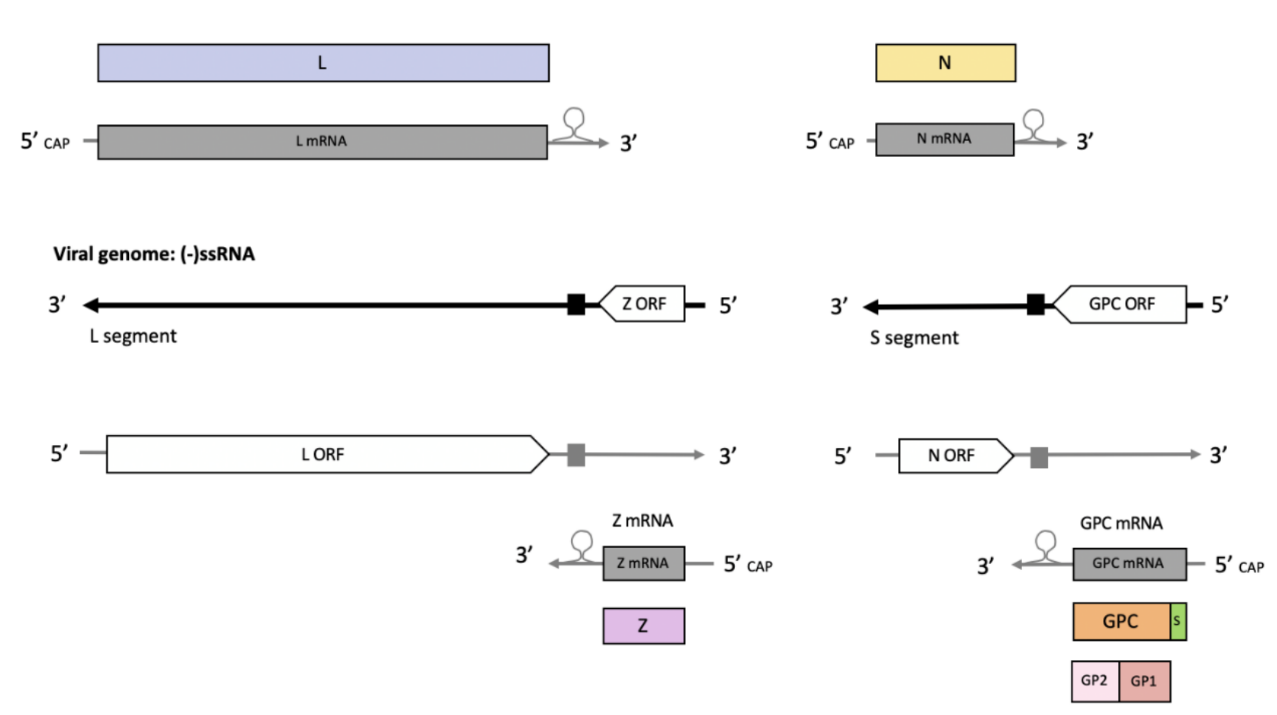
\includegraphics[width=.8\textwidth]{lassa_genome_schematic}
  \caption[Scematic of the LASV genome]{The \gls{lasv} genome is divided into two segments, each containing two different genes. Both segments are ambisenseand contain two oppositely oriented open reading frames separated by an intergenic region. (\textit{Figure credit: Kafetzopoulou 2019} \cite{lianaThesis})}
  \label{fig:lasvGenome}
\end{figure}

%%%%%%%%%%%%%%%%%%%%%%%%%%%%%%%%%%%%%%%%%%%%%%%%%%
% Keep the following \cleardoublepage at the end of this file,
% otherwise \includeonly includes empty pages.
\cleardoublepage

% vim: tw=70 nocindent expandtab foldmethod=marker foldmarker={{{}{,}{}}}
